Jetzt wird es zur praktischen Umsetzung der Signalverarbeitung im Empfänger übergegangen. Der Versuch besteht aus mehreren Teilen, die jeweils verschiedene Aspekte der Signalverarbeitung behandeln.

\section{Vermessung der Sensitivität des Empfängers} %Farhad
\subsection{Vermessung der Ausgangsleistung des Empfängers}
Eine groben Veranschaulichung des Versuchsaufbaus für die Vermessung der Leistung ist in Abbildung \ref{fig:versuchsaufbau} zu sehen. 
Als erstes wird die Sensitivität des Empfängers vermessen. Dazu wird eine zweite Platine (Senderplatine) verwendet, die lediglich als ein single-Tone Sender fungiert. Die Ausgansleistung des Senders wird mit dem Spektrumanalysator als Referenz gemessen. 
\begin{figure}[H]
    \centering
    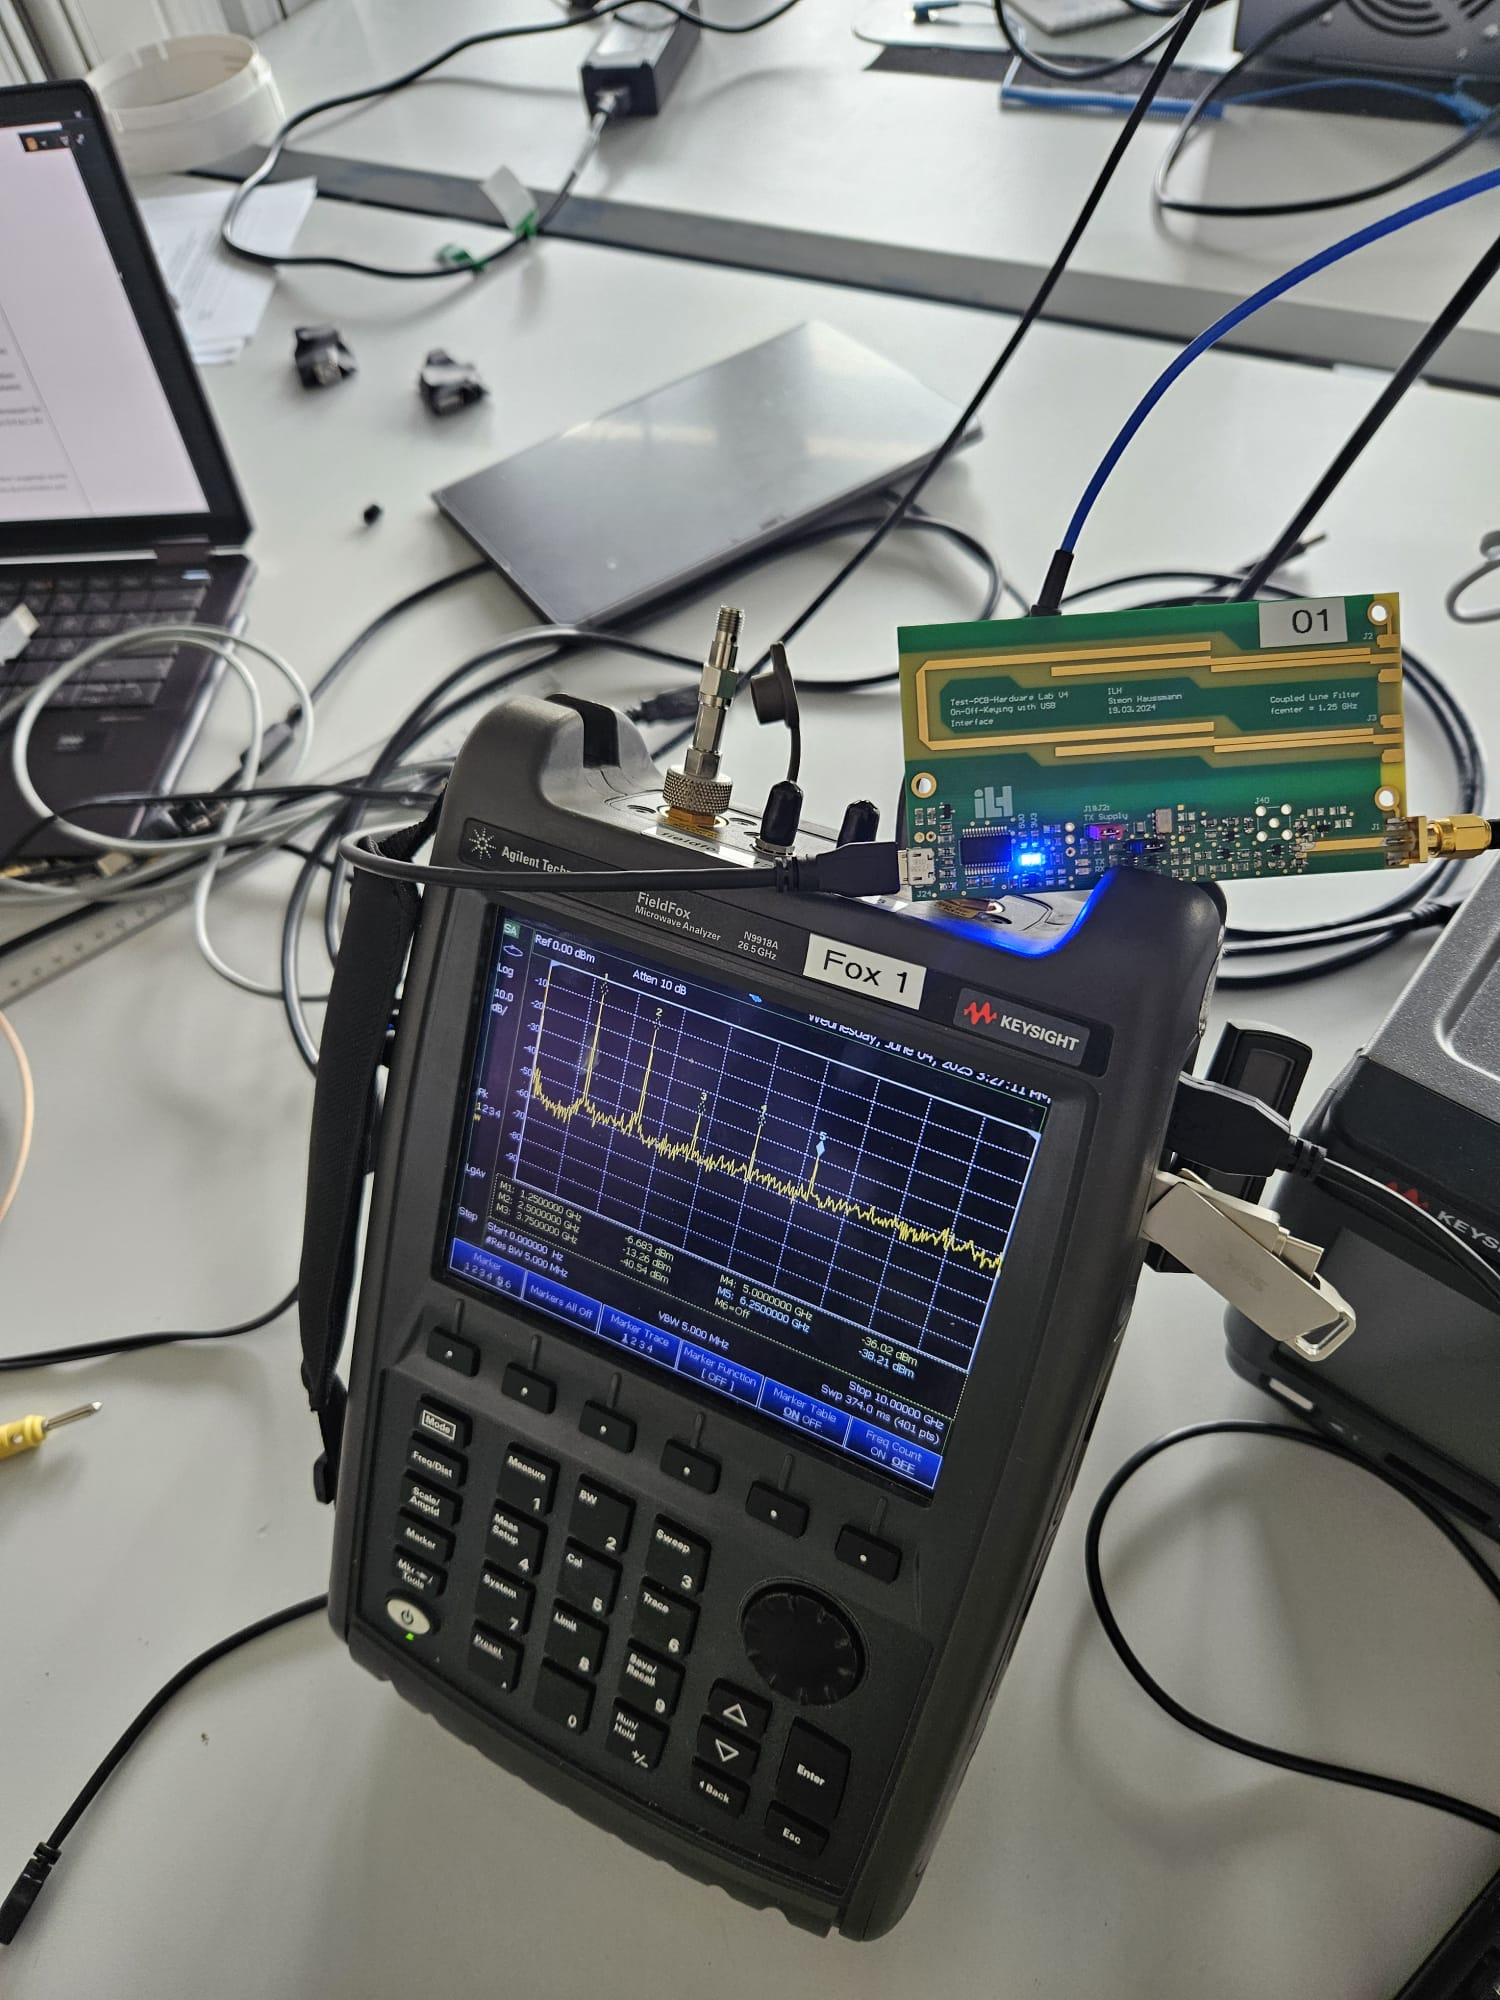
\includegraphics[width=0.5\textwidth]{Pictures/VersuchsaufbauLeistung.jpg}
    \caption{Versuchsaufbau zur Vermessung der Ausgangsleistung des Empfängers}
    \label{fig:versuchsaufbau}
\end{figure}

Insgesamt wurde ein Leistungsspektrum des Senders gemessen, welches in Abbildung \ref{fig:sender} zu sehen ist. Zur genauen Vermessung sind die Werte bei den Harminischen von 1,25 GHz mit Markern versehen, um die genaue Leistung zu bestimmen.

%\begin{figure}[H]
%    \centering
%    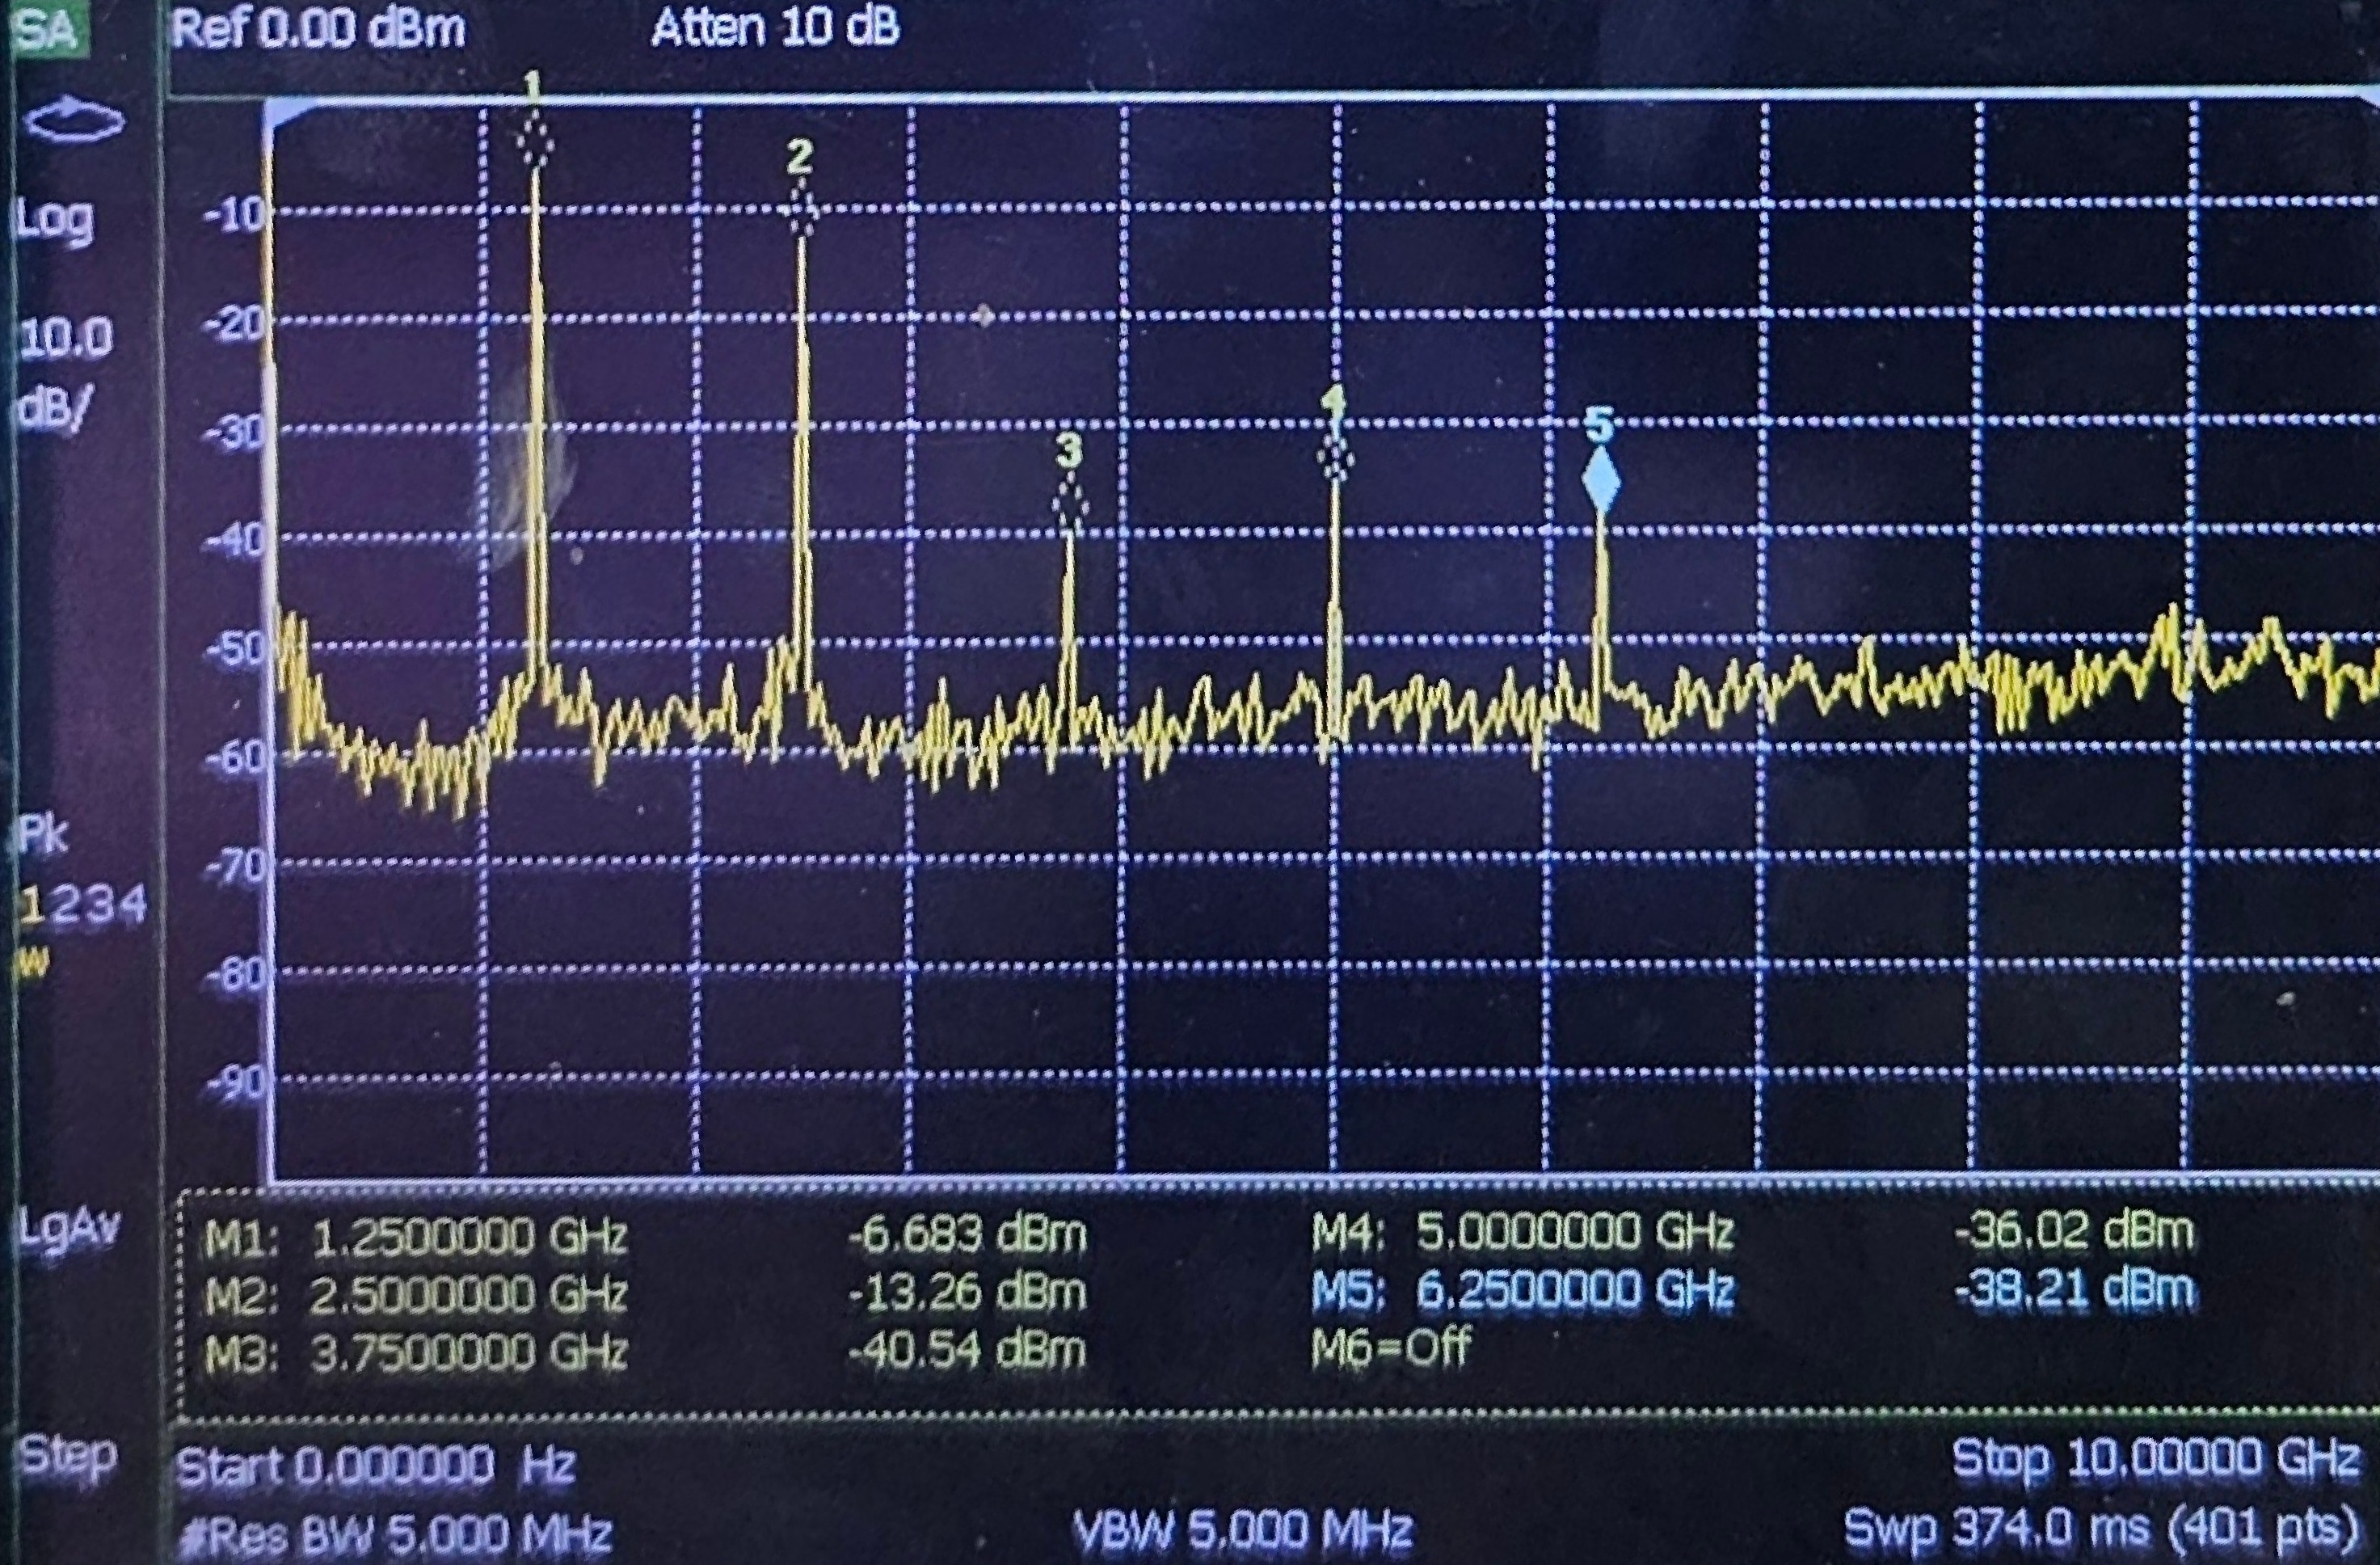
\includegraphics[width=0.8\textwidth]{Pictures/Sender.png}
%    \caption{Leistungsspektrum des Senders}
%    \label{fig:sender}
%\end{figure}

\subsection{Vermessung der Spannung am Kondensator C22}
Die DC-Spannung am Kondensator C22 wird jetzt auf der Empfängerplatine gemessen. Hierbei werden verschiedene Dämpfungsglieder verwenden, um die Leistung des Senders zu variieren. Eine grobe Veranschaulichung des Versuchaufbaus dafür ist in Abbildung \ref{fig:versuchsaufbau2} zu sehen.
\begin{figure}[H]
    \centering
    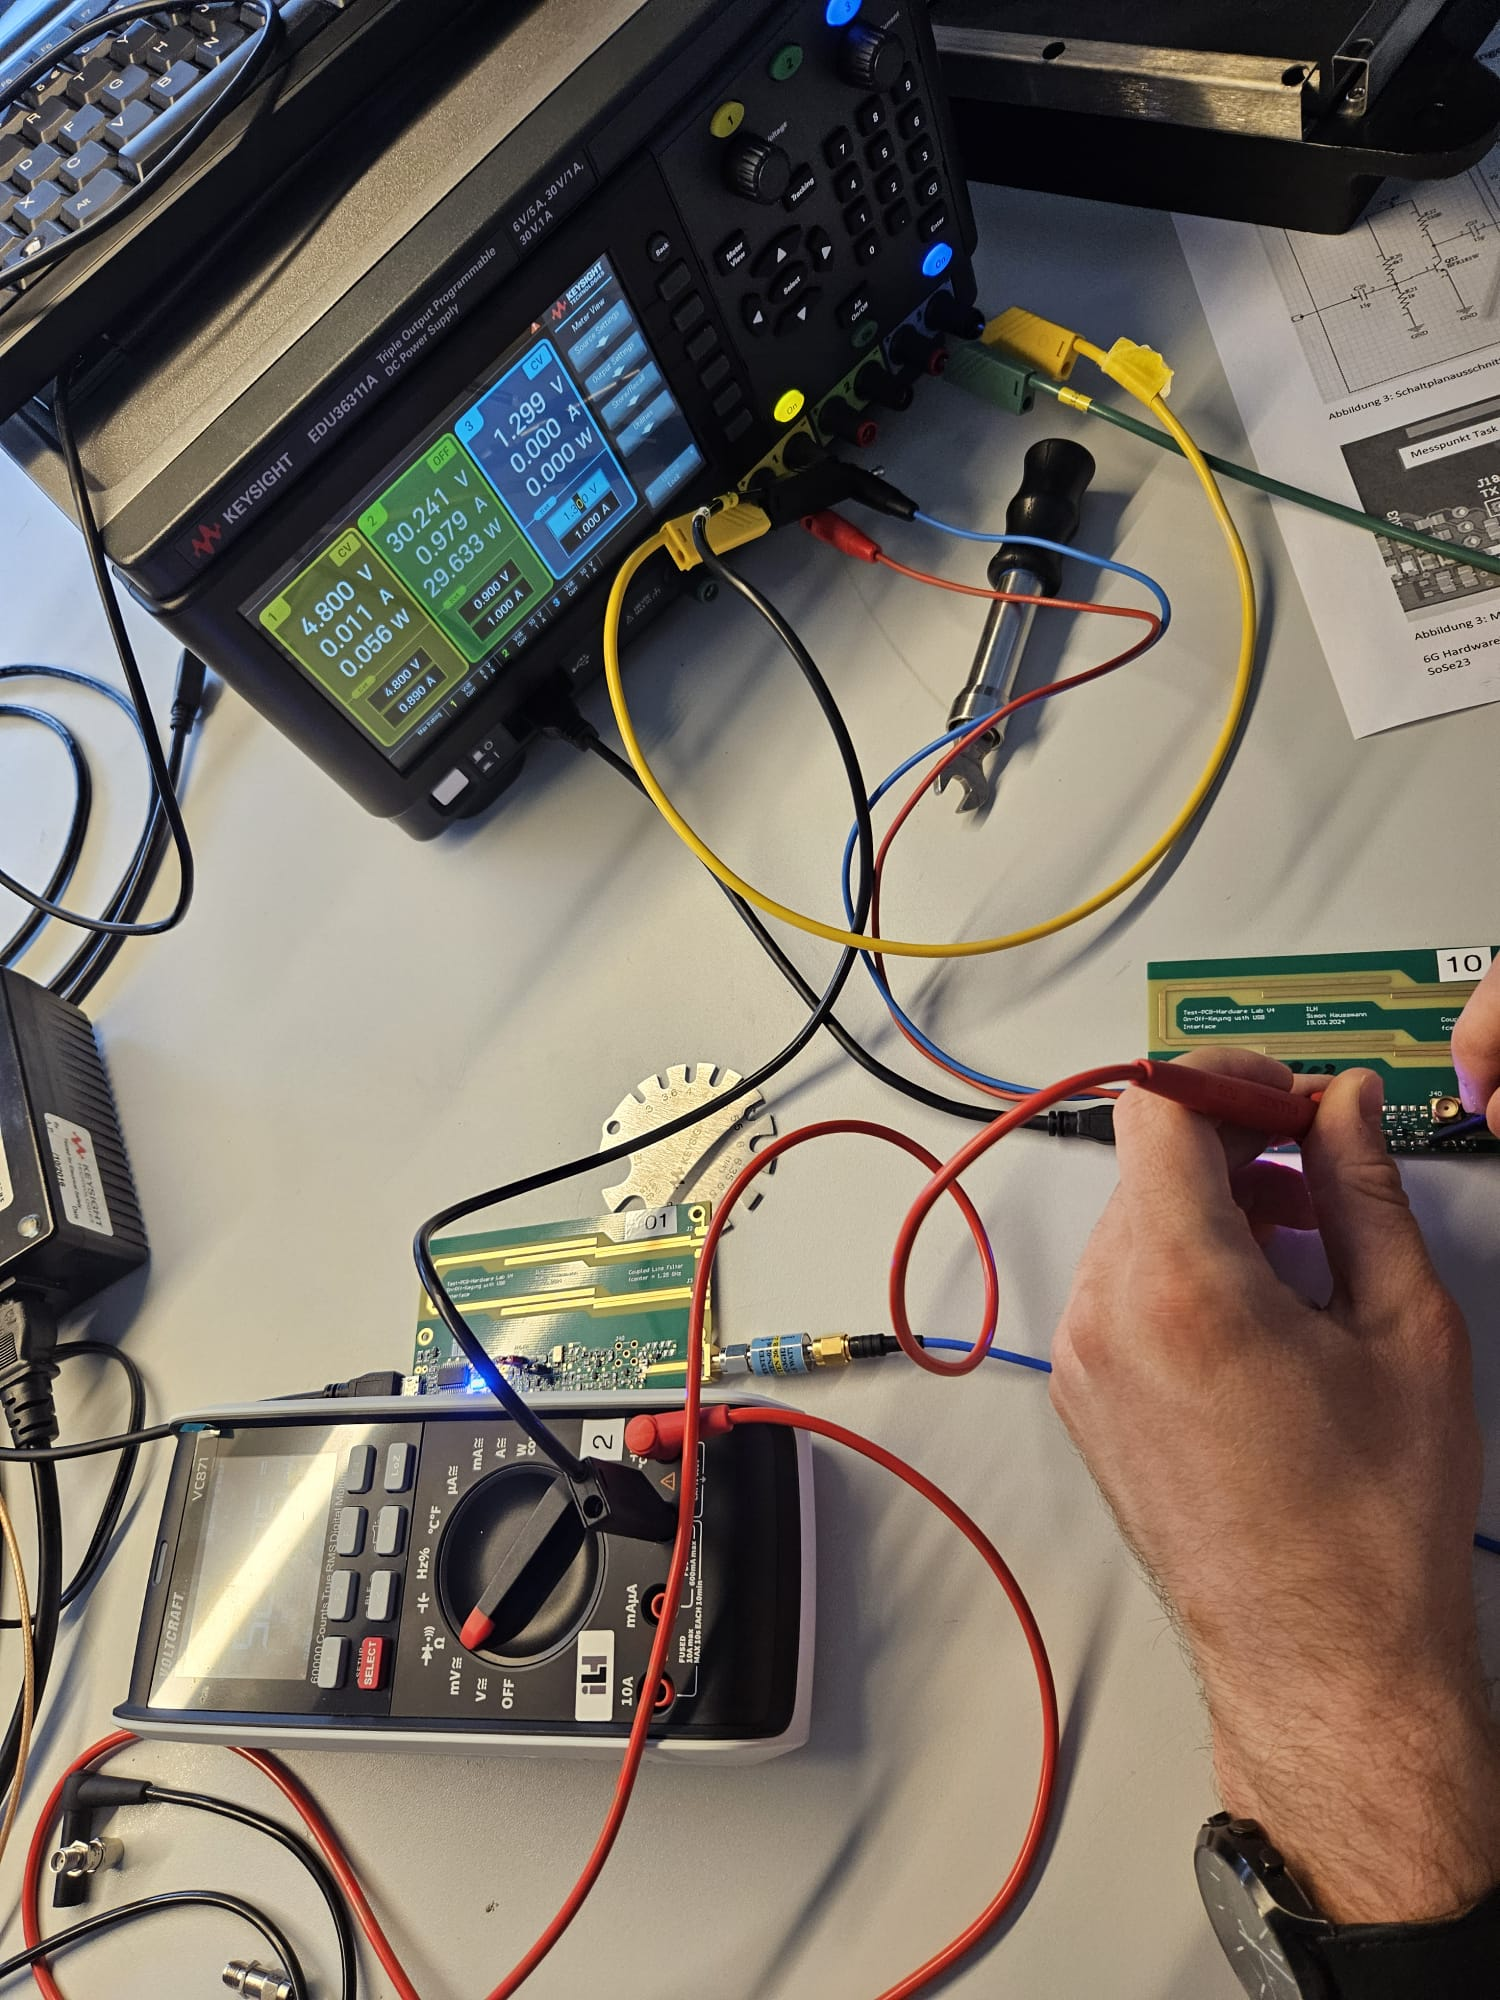
\includegraphics[width=0.5\textwidth]{Pictures/VesuchsaufbauSpannung.jpg}
    \caption{Versuchsaufbau zur Vermessung der Spannung am Kondensator C22}
    \label{fig:versuchsaufbau2}
\end{figure}
Die Spannung am Kondensator C22 wird mit einem Multimeter gemessen. Die Ergebnisse sind in Tabelle \ref{tab:spannung} zu sehen.
\begin{table}[H]
    \centering
    \caption{Messwerte der Spannung am Kondensator C22}
    \begin{tabular}{|c|c|}
        \hline
        Dämpfungsglied & Spannung am C22 [mV] \\ \hline
        0 dB            & 386,47                 \\ \hline
        3 dB            & 383,20                 \\ \hline
        6 dB            & 379,85                 \\ \hline
        10 dB           & 375,10                 \\ \hline
        13 dB           & 372,90                 \\ \hline
        20 dB           & 368,90                 \\ \hline
        26 dB           & 368,27                 \\ \hline
    \end{tabular}
    \label{tab:spannung}
\end{table}

Wie man der Tabelle \ref{tab:spannung} entnehmen kann, fällt die Spannung am Kondensator C22 mit zunehmender Dämpfung des Senders ab. Dies ist zu erwarten, da die Leistung des Senders mit zunehmender Dämpfung verringert wird, was zu einer geringeren Spannung am Kondensator führt.

\subsection{Übertragungsfunktion des Empfängers (Ausgangsspannung/Eingangsleistung)}
Insgesamt stellt es sich heraus, dass diese Schaltung sich wie ein HF-Detektor (Schwellenwertdetektor) funktioniert. Der eingehende Hochfrequenzsignal wird gleichgerichtet und die DC-Spannung am Kondensator C22 ist proportional zur Leistung des eingehenden Signals. 
, also \( P \propto V_\text{in}^2 \), wobei \( V_\text{in} \) die Eingangsspannung ist. Die Beziehung zwischen der Spannung am Kondensator und der Leistung des eingehenden Signals ist quadratisch. Das liegt daran, dass der Eingangssignal des Empfängers hoch genug dafür ist, dass er insgesamt im linearen Bereich arbeitet. 

Hier sind jedoch einige Effekte zu beachten, die die Übertragungsfunktion beeinflussen können. Erstens fleißt aufgrund der Arbeitspunkteinstellung des Transistors Q21 ein Strom durch den Widerstand R26. Die entsprechende Spannung beträgt ungefähr $368,27~mV$ und muss aus der Beziehung herausgerechnet werden, um die Übertragungsfunktion zu erhalten. Außerdem ist ein den Bauteilen der Schaltung charakteristische Konstante \( k \) zu berücksichtigen, die die Übertragungsfunktion beeinflusst. Diese Konstante kann experimentell bestimmt werden.

Die Übertragungsfunktion des Empfängers kann also wie folgt dargestellt werden:
\begin{equation}
    V_\text{out} = k \cdot \sqrt{P_\text{in}} - V_\text{offset}
\end{equation}
wobei \( V_\text{offset} \) die Spannung am Widerstand R26 ist, die den Arbeitspunkt des Transistors Q21 festlegt. 

\section{Operationsverstärkerschaltung} %Lukas
Nun wird mit einer zweiten Spannungsquelle vor der Diode eine Spannung eingespeist und dabei die Transferfunktion
$V_{out}/V_ {in}$ vermessen. Der Spanungsbereich dieser Hilfsspannungsquelle $V_{in}$ wird von 0.9V in 0,01V-Schritten bis 1.4V erhöht.
Da das Protokoll so übersichtlich wie möglich gehalten werden soll, wird in der folgenden Tabelle nur ein kleiner Ausschnitt der
Messwerte gezeigt.
\begin{table}[h]
\centering
\begin{tabular}{|c|c|}
\hline
$V_{\text{in}}$ (V) & $V_{\text{out}}$ (mV) \\
\hline
0{,}9 & 0{,}15571 \\
1{,}0 & 0{,}24478 \\
1{,}1 & 0{,}33307 \\
1{,}2 & 0{,}42666 \\
1{,}3 & 0{,}52090 \\
1{,}4 & 0{,}61620 \\
\hline
\end{tabular}
\caption{Messwerte von $V_{\text{in}}$ und $V_{\text{out}}$ ohne Verstärkung}
\end{table}
\clearpage
Bei genauer Betrachtung der Messwerte wurde offensichtlich das die Platine beschädigt ist. Es findet keine Verstärkung
statt. Daher werden nun im weiteren Verlauf zwei Messungen betrachtet. Eine Messung ohne Verstärkung und eine Messung mit Verstärkung, die von 
unseren Komilitonen (Name?) durchgeführt wurde. Hier werden etwas mehr Messwerte zu einer groben Veranschaulichung benötigt. \\

\begin{table}[h]
\centering
\begin{tabular}{|c|c|}
\hline
$V_{\text{in}}$ (V) & $V_{\text{out}}$ (mV) \\
\hline
0{,}9 & 0{,}039 \\
1{,}0 & 0{,}047\\
1{,}03 & 0{,}077 \\
1{,}06 & 0{,}242 \\
1{,}1 & 0{,}531 \\
1{,}2 & 1{,}258 \\
1{,}3 & 1{,}994 \\
1{,}4 & 2{,}741 \\
\hline
\end{tabular}
\caption{Messwerte von $V_{\text{in}}$ und $V_{\text{out}}$ mit Verstärkung}
\end{table}
In Abbildung 4.3 ist die Transferfunktion $V_{out}/V_ {in}$ dargestellt. Die geplottete Transferfunktion wurde
unter Berücksichtigung aller Messwerte erstellt.\\
(Eingehen auf 7,36 ungefähr 7,8V)





\begin{figure}[H]
    \centering
    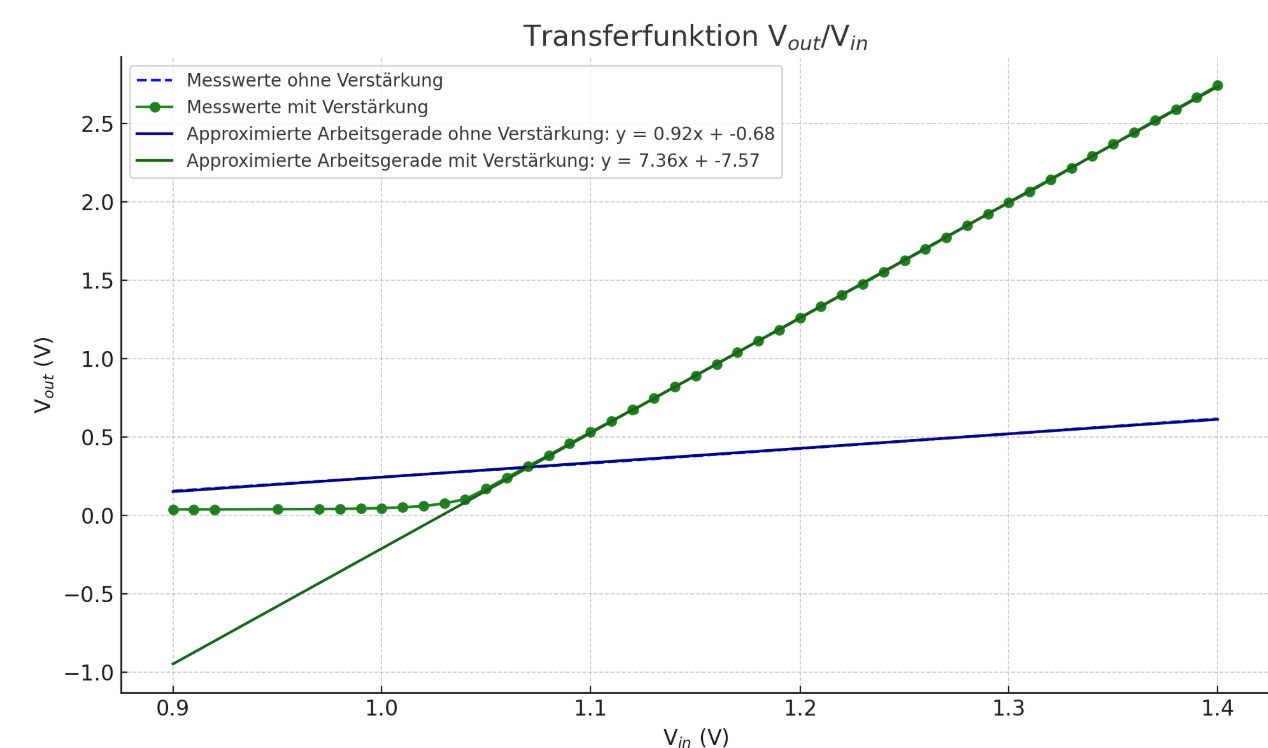
\includegraphics[width=1\textwidth]{Pictures/Transferfunktion.png}
    \caption{Schaltplan des Empfängers}
    \label{fig:opamp_schaltung}
\end{figure}


\section{Komparatorschaltung} %Erik
Zuletzt wird überpfüft ob der Komperator beim angelgen des HF-Tones durchschaltet und somit das übertragen der digitalen Daten funktioniert.
Unsere Messwerte müssen hier nicht betrachtet werden, da der Schaltschwellwert des Kompaarators von
$U_{ref}= 0,79V$ nicht überschritten wird und somit der Komparator nicht schaltet und es auchhhh keinnenS Sinn macht?
Wir beziehen uns hier wieder auf ein Messreihe unserer Komilitonen. In der folgende Tabelle wird die gemessene Spannung 
aufgetragen die vor dem Komparator ankommt und wie sich der Komperator verhält. Das bedeutet welche Ausgangsspannung
der Komparator in Abhängigkeit von der Eingangsspannung hat (LOW und HIGH)

\begin{table}[h]
\centering
\begin{tabular}{cc}
\textbf{Eingangsspannung} & \textbf{Ausgangsspannung} \\
\hline
0{,}811 & 0{,}242 \\
0{,}812 & 0{,}243 \\
0{,}816 & 0{,}244 \\
0{,}820 & 0{,}244 \\
0{,}821 & 0{,}245 \\
0{,}822 & 3{,}298 \\
\end{tabular}
\caption{Messwerte für Eingangsspannung und Ausgangsspannung}
\end{table}

Anhand der Tabelle kann man erkennen, dass der Komparator für Eingangsspannungen unterhalb von 0{,}822\,V auf LOW bleibt. Sobald die Eingangsspannung von 0{,}822\,V überschritten wird, schaltet der Ausgang auf HIGH. Die gemessene Schaltschwelle liegt somit etwas höher als der theoretische Wert $U_{ref} = 0{,}798$\,V bzw. der im Schaltplan angegebene Wert von 0{,}79\,V. Dies kann auf verschiedene Faktoren wie Bauteiltoleranzen oder Messungenauigkeiten zurückzuführen sein. 